Given the goals outlined above, we propose the following experiment as an
initial evaluation of our proposed feasibility prediction approach. We use
model-based GUI test suites as our input suites and Java Swing applications as
Applications Under Test (AUTs). To support execution of these suites, we
develop a scalable and portable execution infrastructure. Below, we elaborate
on the experimental setup and planned analyses.

\subsection{AUTs}

For this initial study, we chose two GUI-based Java Swing applications as
AUTs. While we acknowledge that choice of application platform and technology
may have some effects on experimental outcomes, in our case, Java tooling
for model-based test execution is far ahead of similar tooling for other
domains such as mobile and Web. We consider expansion of AUT domains an item
for future work.

Our first Java Swing application is the JabRef reference manager
\footnote{\url{http://jabref.sourceforge.net/}}, which features a complex
GUI built around extensive data entry and nearly 12 years of
open-source development. Our second application is
ArgoUML\footnote{\url{http://argouml.tigris.org/}}, a largely graphical
GUI-based Java application for constructing diagrams with connected
components. These applications represent real-world examples for model-based
testing. They also draw from multiple domains and use cases as GUI-based
applications.

\subsection{Tools and Execution Infrastructure}
\begin{figure}[ht]
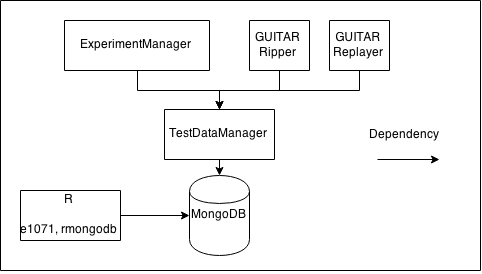
\includegraphics[width=\linewidth]{images/Tools.png}
\caption{Tool stack for experiments: Custom Java tools backed by a MongoDB database}
\label{fig:tools}
\end{figure}

\subsection{Input and Combined Test Suites}

\subsection{Planned Analyses}
